%% KAIS submission -- Springer Nature LaTeX template (sn-jnl). Tables are generated by make_kais.py and
%% inlined by build.py into main.tex.
\documentclass[pdflatex,sn-mathphys-ay]{sn-jnl}

\usepackage{graphicx}
\usepackage{multirow}
\usepackage{amsmath,amssymb,amsfonts}

\usepackage{amsthm}
\usepackage{booktabs}
\usepackage{xcolor}
\usepackage{url}
\usepackage{algorithm}
\usepackage{algorithmicx}
\usepackage{algpseudocode}

\theoremstyle{plain}
\newtheorem{theorem}{Theorem}
\newtheorem{lemma}{Lemma}
\newtheorem{corollary}{Corollary}
\newtheorem{proposition}{Proposition}
\theoremstyle{remark}
\newtheorem{remark}{Remark}

\raggedbottom

\begin{document}

\title{Few-Shot Direction Calibration of Relational and Attribute Statistics for Training-Free Graph Anomaly Detection}

\author*[1]{\fnm{Wasim} \sur{Khan}}\email{wasim.khan@sitpune.edu.in}
\author[2]{\fnm{Shaikh Abdul} \sur{Waheed}}
\author[3]{\fnm{Sujit R.} \sur{Wakchaure}}
\author[4]{\fnm{Anjali Devi} \sur{Patil}}
\author[5]{\fnm{Deepti} \sur{Varshney}}
\author[6]{\fnm{Vajid} \sur{Khan}}

\affil[1]{\orgname{Symbiosis Institute of Technology Pune, Symbiosis International (Deemed University)}, \city{Pune}, \country{India}}
\affil[2]{\orgdiv{Department of Computer Science and Engineering}, \orgname{JSPM University}, \city{Pune}, \country{India}}
\affil[3]{\orgdiv{Department of Computer Engineering}, \orgname{Amrutvahini College of Engineering}, \city{Sangamner}, \country{India}}
\affil[4]{\orgdiv{Department of AIDS}, \orgname{Smt Indira Gandhi College of Engineering}, \city{Navi Mumbai}, \country{India}}
\affil[5]{\orgdiv{Department of Computer Engineering}, \orgname{Ajeenkya D Y Patil School of Engineering}, \city{Pune}, \country{India}}
\affil[6]{\orgdiv{Department of Computer Engineering}, \orgname{Genba Sopanrao Moze College of Engineering}, \city{Pune}, \country{India}}

\abstract{Training-free graph anomaly detectors score nodes with relational statistics, such as neighbour disagreement or triangle participation, and must decide for each statistic whether high or low values are anomalous. We show that this direction decides their performance and cannot be learned without labels. Unlabelled data are consistent with anomalies in either tail of every statistic, and labelled normal nodes, the supervision used by recent generalist detectors, carry little information when anomalies are rare. A few labelled anomalies, by contrast, identify the direction with an error that falls exponentially in their number. Building on these results, we propose few-shot direction calibration (FDC), a training-free method that orients and weights relational and attribute statistics using only $k$ labelled anomalies, with a weight threshold derived from the null distribution of the shots. We evaluate FDC on 16 development graphs and, after freezing the method, on four held-out graphs, against the official implementations of GDN and BWGNN given the same labels. On the development graphs FDC reaches a mean AUROC of 0.800 with ten labelled anomalies (GDN 0.645, BWGNN 0.527). On the held-out graphs it beats both baselines in all 13 graph and shot-size combinations (mean AUROC 0.723 against 0.525 and 0.491; one-sided Wilcoxon $p=0.0001$), and it remains ahead when the baselines also receive a labelled validation set. All protocols were fixed before the corresponding results were seen.}

\keywords{Graph anomaly detection, Few-shot learning, Training-free detection, Identifiability, Positive-unlabelled learning, Pre-registration}

\maketitle

\section{Introduction}\label{sec:intro}

Graph anomaly detection (GAD) identifies nodes whose attributes, connections, or both are unusual relative to the rest of a graph \citep{akoglu2015graph,ma2023comprehensive}. It is used to find fraudulent reviewers, spam accounts and compromised nodes, where labels are scarce and expensive. Most detectors learn a representation of each target graph, by reconstruction \citep{ding2019deep}, contrastive learning \citep{liu2021cola} or affinity maximisation \citep{qiao2023truncated}. Generalist detectors train once on source graphs and transfer to new ones \citep{niu2025unprompt,qiao2025anomalygfm,liu2024arc}. Training-free detectors avoid training altogether and score nodes with relational statistics computed directly on the target graph \citep{zhao2025freegad,wei2026neighbordiv}.

Training-free detectors are cheap, transparent and need no source data. They also rest on a choice that is rarely stated: for every statistic, someone must decide which tail is anomalous. A node whose features disagree with its neighbours is usually suspicious, so neighbour disagreement is scored in its upper tail; a node embedded in few triangles may be suspicious, so triangle participation is scored in its lower tail. These directions are set once and applied to every graph.

We found that these directions decide performance. Our own nine-statistic training-free detector, CoRe-GAD-MSDA, performed well on the graphs it was developed on, reproduced exactly, and still fell below random on several standard benchmarks. The cause was orientation. On graphs with injected clique anomalies, anomalous nodes have \emph{many} triangles, not few; on Weibo, Tolokers and YelpChi, anomalous accounts are \emph{more} similar to their neighbours than normal accounts are. Sixteen label-free rules for choosing directions per graph, fixed in a pre-registered protocol, all failed to generalise, and so did directions chosen from labelled normal nodes. Only labelled anomalies recovered the direction reliably.

This paper turns that observation into a method and explains why it works. Our contributions are as follows.
\begin{enumerate}
\item \textbf{Theory.} We prove that the anomalous direction of a statistic is not identified by unlabelled data, that $m'$ labelled normal nodes leave it undetermined with probability of order $\exp(-m'\pi/(1-\pi))$ when the anomaly rate is $\pi$, and that $k$ labelled anomalies identify it with error at most $\exp(-2k\Delta^2)$, where $\Delta$ is the separation of the statistic (Section~\ref{sec:theory}). The results hold for any fixed graph, without a distributional model.
\item \textbf{Method.} We propose few-shot direction calibration (FDC), which orients and weights relational and attribute statistics using only $k$ labelled anomalies and the unlabelled graph, with no training (Section~\ref{sec:method}). Its weight threshold is the null standard deviation of the shots, and its use of attribute statistics is gated by the number of shots, both as derived in Section~\ref{sec:theory}.
\item \textbf{Evaluation.} We compare FDC with the official code of GDN \citep{ding2021few} and BWGNN \citep{tang2022rethinking} under identical supervision on 16 development graphs, and then on four held-out graphs after freezing the method (Sections~\ref{sec:setup}--\ref{sec:results}). Every protocol and selection rule was fixed and hashed before the corresponding results were computed, and the development history of the method is reported in full.
\end{enumerate}

FDC beats both baselines on the held-out graphs in all 13 graph and shot-size combinations and on 11 to 12 of 15--16 development graphs at each shot size. It is weaker on some organic-anomaly graphs (Questions, Tolokers) and on Facebook, where the official GDN is nearly perfect. We report these cases, a small loss in average precision on the held-out graphs relative to the relational-only variant, and the fact that FDC is not faster than GDN, whose official model is a small linear network.

\section{Related work}\label{sec:related}

\paragraph{Unsupervised and generalist GAD.} Early detectors used ego-network statistics and residual models \citep{10.1007/978-3-642-13672-6_40,ijcai2017p299}. Deep unsupervised detectors reconstruct attributes and structure \citep{ding2019deep}, contrast nodes with their neighbourhoods \citep{liu2021cola,jin2021anemone,zheng2023slgad}, or maximise local affinity \citep{qiao2023truncated,zhang2025gctam}; surveys organise these families \citep{ma2023comprehensive,11048498}. Generalist detectors transfer across graphs: UNPrompt with neighbourhood prompts \citep{niu2025unprompt}, AnomalyGFM with normal and abnormal prototypes \citep{qiao2025anomalygfm}, ARC with in-context learning \citep{liu2024arc}, and ReFi-GAD with relational fingerprints \citep{liu2026refigad}. In their few-shot modes, ARC and AnomalyGFM receive labelled \emph{normal} nodes of the target graph. FreeGAD and NeighborDiv remove training and score nodes with fixed-sign deviations \citep{zhao2025freegad,wei2026neighbordiv}; the orientation problem studied here applies to them directly.

\paragraph{Few-shot and semi-supervised GAD with labelled anomalies.} Deviation networks learn anomaly scores from a few labelled anomalies and unlabelled data by pushing the labelled anomalies away from a Gaussian reference \citep{pang2019deep}. GDN brings this idea to graphs, and Meta-GDN adds meta-learning across auxiliary graphs that share the target's feature space \citep{ding2021few}. Spectral GNNs such as BWGNN are strong supervised detectors when many labels are available \citep{tang2022rethinking}; GADBench compares such detectors in fully and semi-supervised settings \citep{tang2023gadbench}. Our setting, a few labelled anomalies and no labelled normal nodes, is positive--unlabelled learning \citep{elkan2008learning,bekker2020learning}; unlike these methods, FDC has no trainable parameters and uses the labels only to orient and weight a fixed set of statistics.

\paragraph{Evaluation practice.} Evaluation studies in outlier detection have shown that conclusions depend strongly on datasets, measures and protocols \citep{campos2016evaluation,3600270.3602229,tang2023gadbench}. Negative results are under-reported in machine learning \citep{karl2024negative}, and pre-registration guards against analyses tuned after seeing results \citep{nosek2018preregistration}. For comparisons over many datasets we follow the recommendation of \citet{demsar2006statistical} and use the Wilcoxon signed-rank test \citep{wilcoxon1945individual}.

\section{Base detector}\label{sec:detector}

FDC is built on CoRe-GAD-MSDA, a training-free detector developed by the authors and not published elsewhere. Its name refers to its calibrated relational (CoRe) evidence and its multi-statistic direction-aware (MSDA) scoring. Fig.~\ref{fig:detector} gives an overview; we specify the detector fully because FDC changes only its orientation and weighting steps.

\begin{figure}[!ht]
\centering
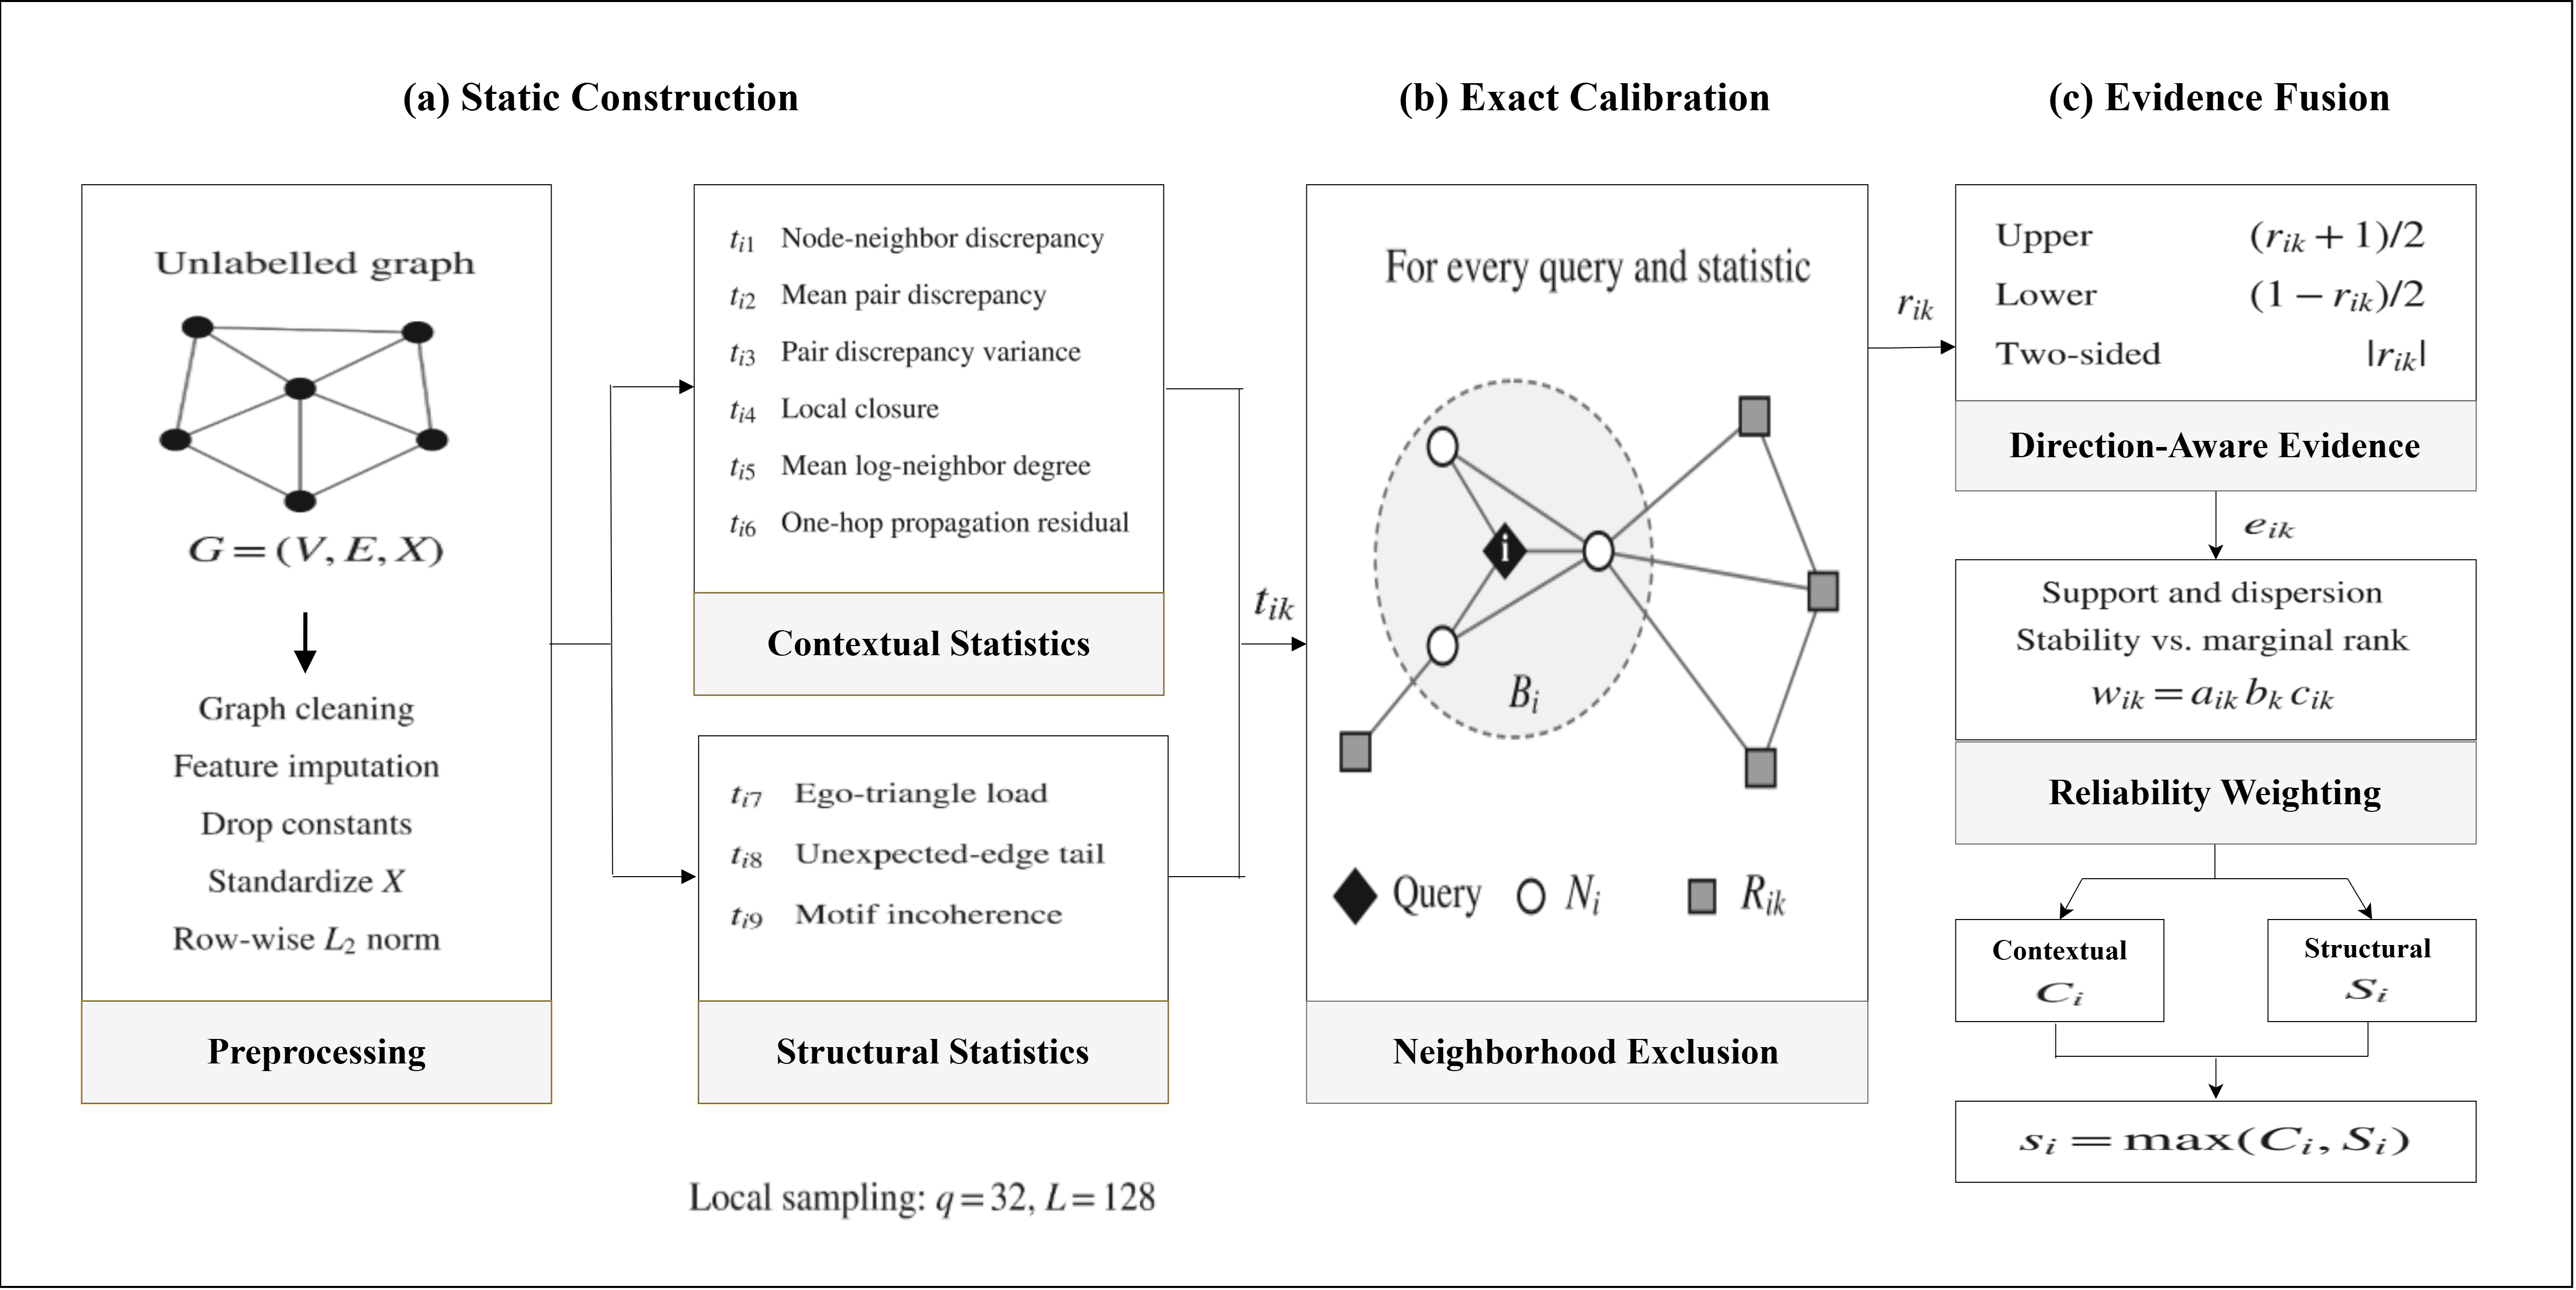
\includegraphics[width=\textwidth]{fig/Fig1_detector.png}
\caption{Overview of the base detector CoRe-GAD-MSDA. Nine statistics are computed per node, calibrated as signed empirical ranks against a reference set that excludes the query and its neighbours, oriented by a tail direction, and fused with label-free reliability weights and a contextual/structural branch maximum. FDC (Section~\ref{sec:method}) replaces the fixed orientation with one calibrated from labelled anomalies and adds attribute statistics.}
\label{fig:detector}
\end{figure}

\paragraph{Setting and preprocessing.} Let $\mathcal{G}=(\mathcal{V},\mathcal{E},\mathbf{X})$ be an undirected attributed graph with $n$ nodes, binary adjacency matrix $\mathbf{A}$ without self-loops, degree matrix $\mathbf{D}$ and features $\mathbf{X}\in\mathbb{R}^{n\times d}$; $\mathcal{N}_i$ and $d_i=|\mathcal{N}_i|$ are the neighbours and degree of node $v_i$. Non-finite feature entries are replaced by their column median, constant columns are removed, each column is standardised and each row is scaled to unit norm. We write $\tilde{\mathbf{x}}_i$ for the result and $\delta_{uv}=1-\tilde{\mathbf{x}}_u^{\top}\tilde{\mathbf{x}}_v$ for the cosine dissimilarity of two nodes.

\paragraph{Relational statistics.} For each node the detector computes nine statistics (Table~\ref{tab:stats}). To bound cost, $\widehat{\mathcal{N}}_i$ is $\mathcal{N}_i$ if $d_i\le q$ and otherwise a uniform sample of $q=32$ neighbours, and $\widehat{\mathcal{P}}_i$ is the set of unordered neighbour pairs if there are at most $L=128$ of them and otherwise a uniform sample of $L$ pairs. The six contextual statistics are
\begin{align}
t_{i1}&=\frac{1}{|\widehat{\mathcal{N}}_i|}\sum_{j\in\widehat{\mathcal{N}}_i}\delta_{ij}, &
t_{i2}&=\frac{1}{|\widehat{\mathcal{P}}_i|}\sum_{(u,v)\in\widehat{\mathcal{P}}_i}\delta_{uv}, \nonumber\\
t_{i3}&=\frac{1}{|\widehat{\mathcal{P}}_i|}\sum_{(u,v)\in\widehat{\mathcal{P}}_i}\big(\delta_{uv}-t_{i2}\big)^2, &
t_{i4}&=\frac{1}{|\widehat{\mathcal{P}}_i|}\sum_{(u,v)\in\widehat{\mathcal{P}}_i}A_{uv}, \nonumber\\
t_{i5}&=\frac{1}{d_i}\sum_{j\in\mathcal{N}_i}\log(1+d_j), &
t_{i6}&=1-\cos\big(\tilde{\mathbf{x}}_i,\mathbf{h}_i\big),\quad \mathbf{H}=(\mathbf{D}+\mathbf{I})^{-1}(\mathbf{A}+\mathbf{I})\tilde{\mathbf{X}}.
\end{align}
With $\mathcal{T}_i$ the neighbour pairs that close a triangle with $v_i$ and $\mathcal{U}_i$ the $\lceil\sqrt{d_i}\rceil$ neighbours with the largest $\delta_{ij}$, the three structural statistics are
\begin{equation}
t_{i7}=\frac{|\mathcal{T}_i|}{d_i}, \qquad
t_{i8}=\frac{1}{|\mathcal{U}_i|}\sum_{j\in\mathcal{U}_i}\delta_{ij}, \qquad
t_{i9}=\frac{1}{|\mathcal{T}_i|}\sum_{(u,v)\in\mathcal{T}_i}\frac{\delta_{iu}+\delta_{iv}+\delta_{uv}}{3}.
\end{equation}
A statistic that is undefined for a node (for example $t_{i9}$ for a node in no triangle) is marked missing for that node. On dense graphs, triangle counts and motif sums are computed exactly with sparse matrix identities in row blocks.

\begin{table}[!ht]
\caption{Relational statistics of the base detector and their fixed directions (U: upper tail anomalous; L: lower tail; 2: two-sided).}
\label{tab:stats}
\footnotesize
\begin{tabular}{@{}llll@{}}
\toprule
Branch & Statistic & Symbol & Fixed direction \\
\midrule
Contextual & Node--neighbour discrepancy & $t_1$ & U \\
 & Mean neighbour-pair discrepancy & $t_2$ & U \\
 & Variance of neighbour-pair discrepancy & $t_3$ & U \\
 & Local closure & $t_4$ & L \\
 & Mean log-neighbourhood degree & $t_5$ & 2 \\
 & One-hop propagation residual & $t_6$ & U \\
\midrule
Structural & Triangle load & $t_7$ & L \\
 & Unexpected-edge tail & $t_8$ & U \\
 & Motif incoherence & $t_9$ & U \\
\botrule
\end{tabular}
\end{table}

\paragraph{Rank calibration.} Let $\mathcal{V}_j$ be the nodes for which statistic $j$ is defined and $\mathcal{R}_{ij}=\mathcal{V}_j\setminus(\{i\}\cup\mathcal{N}_i)$ the reference set of node $i$, of size $m_{ij}$. The neighbourhood-excluded signed midrank is
\begin{equation}\label{eq:rank}
r_{ij}=\frac{2}{m_{ij}}\Big(\sum_{l\in\mathcal{R}_{ij}}\mathbb{1}[t_{lj}<t_{ij}]+\tfrac12\sum_{l\in\mathcal{R}_{ij}}\mathbb{1}[t_{lj}=t_{ij}]\Big)-1\in[-1,1],
\end{equation}
and $M_{ij}=1$ if $t_{ij}$ is defined and $m_{ij}>0$, else $0$. The graph-wide signed midrank $\bar r_{ij}$ is defined in the same way with $\mathcal{R}_{ij}$ replaced by $\mathcal{V}_j$.

\paragraph{Orientation, weighting and fusion.} A tail direction $\theta_j\in\{\text{upper},\text{lower},\text{two-sided}\}$ turns a rank into evidence
\begin{equation}\label{eq:orient}
e_{ij}=M_{ij}\cdot\begin{cases}(1+r_{ij})/2 & \theta_j=\text{upper},\\ (1-r_{ij})/2 & \theta_j=\text{lower},\\ |r_{ij}| & \theta_j=\text{two-sided}.\end{cases}
\end{equation}
Each coordinate receives a label-free reliability weight $\omega_{ij}=a_{ij}b_jc_{ij}$, the product of a support factor $a_{ij}=M_{ij}\min(1,m_{ij}/\max(n_j^{*}-1,1))$ with $n_j^*=\sum_iM_{ij}$, a dispersion factor $b_j=\min(1,\mathrm{IQR}\{e_{ij}\}/0.5)$, and a stability factor $c_{ij}=M_{ij}\max(0,1-|r_{ij}-\bar r_{ij}|/2)$. The score is the larger of the weighted mean evidence of the contextual statistics ($j\le6$) and of the structural statistics ($j\ge7$),
\begin{equation}\label{eq:fusion}
s_i=\max\Big(\frac{\sum_{j\le6}\omega_{ij}e_{ij}}{\sum_{j\le6}\omega_{ij}},\;\frac{\sum_{j\ge7}\omega_{ij}e_{ij}}{\sum_{j\ge7}\omega_{ij}}\Big),
\end{equation}
with an empty branch scoring 0. With the fixed directions of Table~\ref{tab:stats}, the detector needs no labels and has no trainable parameters.

\section{Why fixed or label-free directions fail}\label{sec:motivation}

This section summarises the evidence that motivated FDC. It comes from an earlier study of the base detector on 21 standard benchmark files, which we reproduce here only as far as it is needed.

\paragraph{Reproduction.} The base detector's original results reproduce exactly (164 of 164 released AUROC and AP values), and the official UNPrompt and AnomalyGFM reruns are close to their published values. The failures below are therefore not implementation artefacts.

\subsection{The anomalous direction depends on the anomaly mechanism}\label{sec:rq3}

Fig.~\ref{fig:diag} shows, for each graph and statistic, the AUROC of the oriented statistic on its own. On every graph with injected clique anomalies, triangle load is reversed: planted cliques give anomalous nodes unusually many triangles. On Weibo, Tolokers and YelpChi, the discrepancy statistics and the propagation residual are reversed: anomalous accounts are more similar to their neighbours than normal accounts are, a pattern consistent with camouflage. The same nine statistics that score below random on Weibo with the fixed directions reach 0.824 AUROC when oriented two-sided. No fixed choice of directions works on all graphs.

\begin{figure}[!ht]
\centering
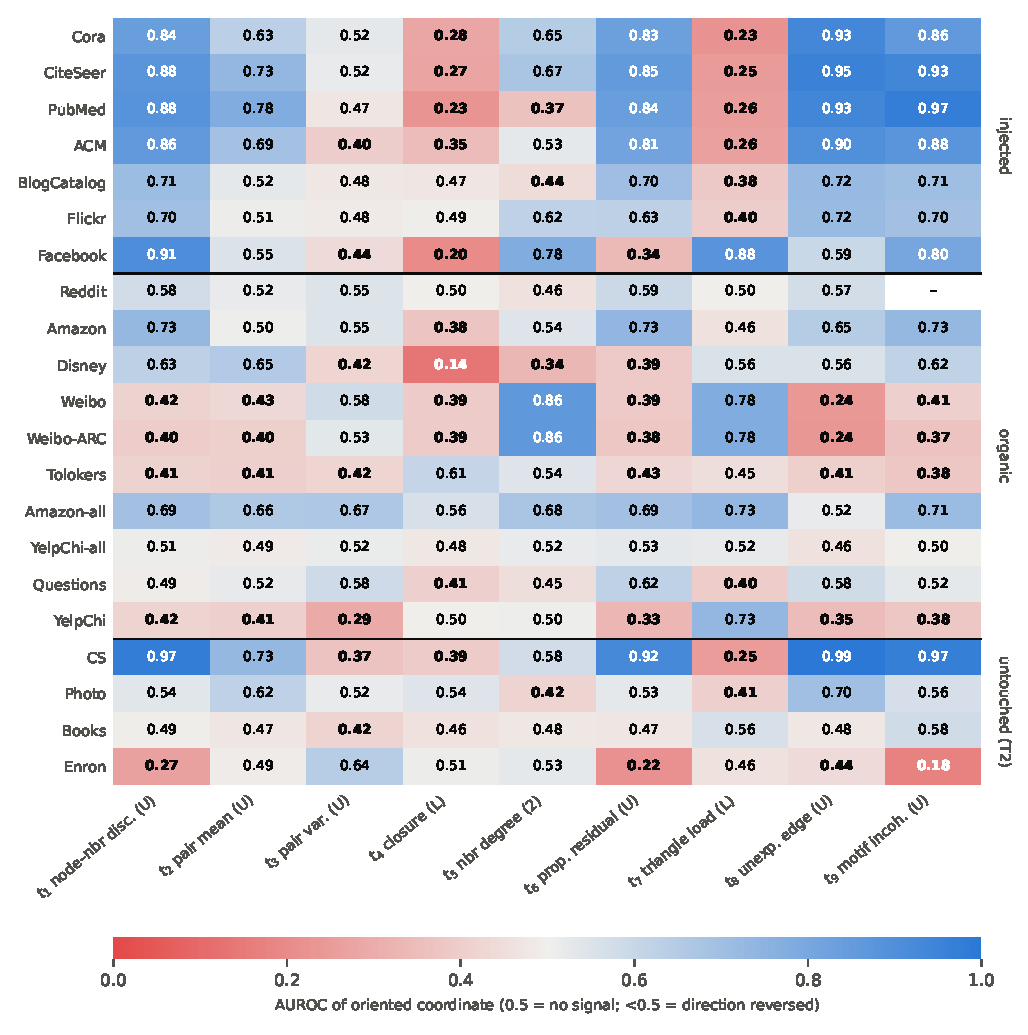
\includegraphics[width=\textwidth]{fig/Fig2_direction_diagnostic.pdf}
\caption{AUROC of each statistic of the base detector on its own, in its fixed direction, averaged over five seeds. Blue: the fixed direction separates anomalies; red: it is reversed. Bold values are below 0.45. Motif incoherence is undefined on Reddit, which has no triangles.}
\label{fig:diag}
\end{figure}

\subsection{Label-free rules do not generalise}\label{sec:rq4}

Before running them, we fixed 16 rules for choosing each statistic's direction from unlabelled data: two references (fixed directions, all two-sided), twelve rules based on the skewness of each statistic, and two consensus rules that align each statistic with the others. The rule with the best development utility, a consensus rule, was frozen and tested. It improved four untouched graphs but lowered mean AUROC on the other test graphs from 0.672 to 0.616, collapsing on Facebook, Flickr and YelpChi. All twelve skewness rules were below random on average, and a representative skewness rule chose the anomalous direction in only 31\% of decisive cases.

\subsection{Labelled normal nodes do not help; labelled anomalies do}\label{sec:rq5}

Fig.~\ref{fig:recovery} shows how often each source of information chooses the direction in which a statistic actually separates anomalies, over 510 decisive statistic--graph--seed cases. Fixed directions are right in 56\% of cases and the consensus rule in 62\%. A rule using $k$ labelled normal nodes, the supervision of ARC and AnomalyGFM, does not improve with $k$ (59\%, 60\% and 54\% for $k=1,5,10$); with ten normal shots the base detector's mean AUROC on ARC's eight test graphs fell from 0.704 to 0.586. Labelled anomalies behave differently: one labelled anomaly with one normal node already gives 68\%, and ten of each give 75\%. FDC is designed to exploit this asymmetry, and Section~\ref{sec:theory} explains it.

\begin{figure}[!ht]
\centering
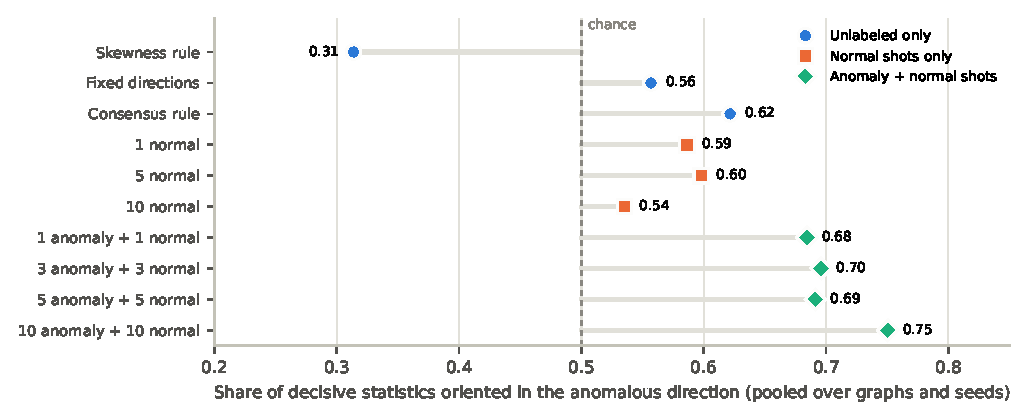
\includegraphics[width=\textwidth]{fig/Fig4_direction_recovery.pdf}
\caption{Share of decisive statistics oriented in their anomalous direction, pooled over graphs and seeds. Only labelled anomalies move the share well above chance.}
\label{fig:recovery}
\end{figure}

% ---------------------------------------------------------------------------
% Theory section. Requires amsmath, amssymb, amsthm and the environments
% theorem, lemma, proposition, corollary, remark (declared in the preamble).
% Proofs are in theory_appendix.tex.
% ---------------------------------------------------------------------------
\section{When can the anomalous direction be identified?}\label{sec:theory}

This section explains the empirical pattern of Sections~\ref{sec:rq3}--\ref{sec:rq5}: label-free rules fail, labelled normal nodes barely help, and a few labelled anomalies are enough. The results are stated for a single relational or attribute statistic on a fixed graph, so they hold without any distributional model of the graph. Proofs are given in Appendix~\ref{app:proofs}.

\subsection{Setting}

Let $G$ be a graph with node set $V$, $|V| = n$, and let $\mathcal{A} \subset V$ be the anomalous nodes, $|\mathcal{A}| = m$, with contamination $\pi = m/n$; $\mathcal{N} = V \setminus \mathcal{A}$ are the normal nodes. A statistic assigns a value $t_i$ to every node. Its \emph{graph-wide rank position} is
\begin{equation}\label{eq:rankpos}
U_i \;=\; \frac{1}{n}\sum_{l \in V}\Big(\mathbb{1}[t_l < t_i] + \tfrac12\,\mathbb{1}[t_l = t_i]\Big) \in (0,1),
\end{equation}
which equals $(r_i + 1)/2$ for the graph-wide signed midrank $r_i$ used by the detector. Write
\begin{equation}
\mu = \frac{1}{m}\sum_{i \in \mathcal{A}} U_i, \qquad
\mathrm{AUC} = \frac{1}{m\,(n-m)}\sum_{i \in \mathcal{A}}\sum_{l \in \mathcal{N}}\Big(\mathbb{1}[t_l < t_i] + \tfrac12\,\mathbb{1}[t_l = t_i]\Big),
\end{equation}
so $\mathrm{AUC}$ is the AUROC obtained by scoring nodes with the upper tail of the statistic. The upper tail is the anomalous direction if $\mathrm{AUC} > \tfrac12$ and the lower tail if $\mathrm{AUC} < \tfrac12$.

\begin{lemma}[Direction is the sign of the mean rank position]\label{lem:sign}
$\mu - \tfrac12 = (1-\pi)\,(\mathrm{AUC} - \tfrac12)$. Hence the upper tail is anomalous if and only if $\mu > \tfrac12$, and the \emph{direction margin}
\[ \Delta = |\mu - \tfrac12| = (1-\pi)\,|\mathrm{AUC} - \tfrac12| \]
measures how strongly the statistic separates anomalies in its anomalous direction.
\end{lemma}

The lemma matters because $\mu$ can be estimated from labelled anomalies alone, using the whole unlabelled graph as reference: no labelled normal node is needed.

\subsection{Unlabelled data do not identify the direction}

A \emph{label-free rule} is any procedure, possibly randomised, whose output depends on the graph, its features and the statistics, but not on any label. All 16 rules of Section~\ref{sec:rq4} are of this kind.

\begin{theorem}[Label-free non-identifiability]\label{thm:nonid}
Let the statistic take distinct values and let $1 \le m < n/2$. Let $\mathcal{A}_{\uparrow}$ be the $m$ nodes with the largest values and $\mathcal{A}_{\downarrow}$ the $m$ nodes with the smallest. Labelling $\mathcal{A}_{\uparrow}$ as anomalous gives $\mathrm{AUC} = 1$; labelling $\mathcal{A}_{\downarrow}$ gives $\mathrm{AUC} = 0$. Both labellings have the same contamination and leave the input of every label-free rule unchanged, so every label-free rule chooses the wrong direction with probability at least $\tfrac12$ under one of them.
\end{theorem}

Theorem~\ref{thm:nonid} is elementary, but it fixes what a label-free rule can and cannot do. Skewness, consensus and similar rules succeed only when the unknown labelling mechanism happens to place anomalies in the tail the rule favours. That is an assumption about how anomalies arise, not something the data can confirm. The benchmarks contain both mechanisms: injected clique anomalies sit in the upper tail of triangle statistics, while organic camouflaged anomalies sit in the lower tail of neighbour disagreement (Section~\ref{sec:rq3}). This is why no fixed label-free rule transferred.

\subsection{Labelled normal nodes are weak evidence}

Labelled normal nodes add information, but very little when anomalies are rare. Suppose $m'$ normal nodes are drawn uniformly without replacement from $\mathcal{N}$ and revealed.

\begin{theorem}[Normal shots]\label{thm:normal}
In the setting of Theorem~\ref{thm:nonid}, assume $n \ge 2m + m'$. Every rule that uses the graph and $m'$ labelled normal nodes chooses the wrong direction, under one of the two labellings, with probability at least
\[
\tfrac12\,q, \qquad
q = \prod_{i=0}^{m'-1}\frac{n-2m-i}{\,n-m-i\,} \;\ge\; \Big(1 - \frac{m}{\,n-m-m'+1\,}\Big)^{m'} \;\approx\; \exp\!\Big(-\frac{m'\pi}{1-\pi}\Big).
\]
\end{theorem}

To push this worst-case error below $\varepsilon$, roughly $m' \ge \frac{1-\pi}{\pi}\ln\frac{1}{2\varepsilon}$ normal nodes are required. With $\pi = 0.05$ and $\varepsilon = 0.1$ this is about 31 labelled normal nodes for a single statistic. With the $m' = 10$ normal shots used by ARC and AnomalyGFM, the bound is between $0.15$ and $0.39$ on the 14 of the 16 development graphs with $\pi < 0.11$. This agrees with the near-chance direction recovery from normal shots reported in Section~\ref{sec:rq5}. The reason is an asymmetry: when anomalies are rare, normal nodes look like the graph as a whole, so they say little about which tail the few anomalies occupy.

\subsection{A few labelled anomalies identify the direction}

Now suppose $k$ anomalies are drawn uniformly without replacement from $\mathcal{A}$ and revealed. The calibration rule estimates $\mu$ by the mean rank position of the shots,
\[
\hat\mu = \frac1k \sum_{s=1}^{k} U_{a_s},
\]
and chooses the upper tail if $\hat\mu > \tfrac12$ and the lower tail otherwise. The mean of $\hat\mu$ is $\mu$, and each $U_{a_s}$ lies in $(0,1)$.

\begin{theorem}[Anomaly shots]\label{thm:anomaly}
Let $\Delta > 0$ be the direction margin of Lemma~\ref{lem:sign} and $\sigma^2 = \frac1m \sum_{i \in \mathcal{A}} (U_i - \mu)^2$ the spread of the anomalies' rank positions. The probability that the calibration rule chooses the wrong direction satisfies
\[
\Pr[\text{wrong direction}] \;\le\; \min\left\{ \exp\!\big(-2k\Delta^2\big),\;
\exp\!\left(-\frac{k\Delta^2}{2\sigma^2 + 2\Delta/3}\right)\right\}.
\]
\end{theorem}

\begin{corollary}[How many anomalies to label]\label{cor:k}
If $J$ statistics all have margin at least $\Delta_{\min}$, all their directions are correct with probability at least $1-\varepsilon$ once
\[
k \;\ge\; \frac{\ln(J/\varepsilon)}{2\,\Delta_{\min}^{2}}.
\]
\end{corollary}

The contrast with Theorem~\ref{thm:normal} is sharp. In the two extreme labellings of Theorem~\ref{thm:nonid}, a single labelled anomaly reveals the direction exactly, while $m'$ normal nodes leave it undetermined with probability close to $\exp(-m'\pi/(1-\pi))$. In general the error with anomaly shots decays exponentially in $k$ at a rate set by $\Delta$, which depends on the contamination only through the factor $1-\pi$. With labelled normal nodes, the worst-case rate is throttled by $\pi$ itself.

\subsection{Choosing which statistics to trust}

With few shots, some statistics look separating by chance. The method therefore weights statistic $j$ by $w_j = \max(0,\ \hat s_j - \tau_k)$. Here $\hat s_j$ is the estimated separation of its chosen tail and $\tau_k = 1/\sqrt{12k}$.

\begin{proposition}[Null calibration of $\tau_k$]\label{prop:tau}
If the $k$ shots are a uniform random sample of nodes with respect to statistic $j$ (no anomaly signal), then for each of the upper, lower and two-sided evidences, the shot mean has expectation $\tfrac12 + O(1/n)$ and standard deviation at most $1/\sqrt{12k} = \tau_k$. If instead statistic $j$ has margin $\Delta_j > \tau_k$, it keeps a positive weight with probability at least $1 - \exp\!\big(-2k(\Delta_j - \tau_k)^2\big)$.
\end{proposition}

Thus $\tau_k$ is one null standard deviation: statistics whose apparent separation is within the noise level of $k$ shots are switched off. Statistics with a real margin above that level are retained with probability approaching one exponentially fast. The same calculation explains the $k$-gate of the final method. At $k = 1$ and $k = 2$, $\tau_k \ge 0.20$, and with $k = 1$ a statistic without any signal still passes this threshold with probability at least $0.42$. Among the $2p$ attribute statistics, many would therefore be retained by chance, so they are used only from $k = 3$ onwards.

\subsection{Empirical check}

Table~\ref{tab:bound} compares the observed direction error of the calibration rule with Theorem~\ref{thm:anomaly}, using the exact $\Delta$ and $\sigma^2$ of each statistic computed from all labels. It pools 9 relational statistics, 16 development graphs and 5 seeds. The observed error never exceeds either bound. Both bounds are conservative: for margins above $0.2$, no error was observed at $k = 10$, while Hoeffding's bound allows $35\%$ and Bernstein's $16\%$. The variance-adaptive Bernstein bound is the tighter of the two throughout. Statistics with margin below $0.05$ are close to a coin flip at every $k$, as the theory predicts; the weight threshold of Proposition~\ref{prop:tau} is designed to discard exactly these.

\begin{table}[t]
\caption{Observed direction error of the anomaly-shot calibration rule against the bounds of Theorem~\ref{thm:anomaly}. Rows pool statistics by their margin $\Delta$; $n$ is the number of (statistic, graph, seed) cases. Development graphs only.}\label{tab:bound}
\centering\small
\begin{tabular}{@{}cl rrrr@{}}
\toprule
$k$ & $\Delta$ & $n$ & Observed & Hoeffding & Bernstein \\
\midrule
1  & $(0.00, 0.05]$ & 172 & 0.494 & 0.999 & 0.997 \\
   & $(0.10, 0.20]$ & 155 & 0.361 & 0.956 & 0.915 \\
   & $(0.30, 0.50]$ &  99 & 0.030 & 0.760 & 0.630 \\
3  & $(0.00, 0.05]$ & 182 & 0.467 & 0.996 & 0.989 \\
   & $(0.10, 0.20]$ & 158 & 0.152 & 0.876 & 0.770 \\
   & $(0.30, 0.50]$ & 104 & 0.019 & 0.444 & 0.258 \\
5  & $(0.00, 0.05]$ & 178 & 0.421 & 0.994 & 0.982 \\
   & $(0.10, 0.20]$ & 138 & 0.188 & 0.795 & 0.647 \\
   & $(0.30, 0.50]$ & 100 & 0.000 & 0.259 & 0.108 \\
10 & $(0.00, 0.05]$ & 178 & 0.478 & 0.987 & 0.965 \\
   & $(0.10, 0.20]$ & 139 & 0.072 & 0.639 & 0.429 \\
   & $(0.20, 0.30]$ & 121 & 0.000 & 0.351 & 0.163 \\
   & $(0.30, 0.50]$ & 100 & 0.000 & 0.073 & 0.015 \\
\bottomrule
\end{tabular}
\end{table}

\section{Few-shot direction calibration}\label{sec:method}

FDC receives a graph and a set $\mathcal{S}$ of $k$ labelled anomalies; all other nodes are unlabelled. It orients and weights a set of statistics using $\mathcal{S}$ and the graph-wide ranks of Section~\ref{sec:detector}, and it has no trainable parameters. Algorithm~\ref{alg:fdc} summarises it.

\paragraph{Statistics.} FDC uses the nine relational statistics of Section~\ref{sec:detector} and $2p$ attribute statistics, $p=\min(16,d-1)$. Let $\mathbf{Z}\in\mathbb{R}^{n\times p}$ be a low-dimensional summary of the features: the first $p$ principal components of the column-standardised features when $d\le64$ and at least 30\% of the feature entries are non-zero, and otherwise a truncated singular value decomposition of the row-normalised features. The attribute statistics of node $i$ are its own components $z_{i1},\dots,z_{ip}$ and the mean of its neighbours' components, $\frac{1}{d_i}\sum_{l\in\mathcal{N}_i}z_{l1},\dots$ (zero for isolated nodes). Attribute statistics are valid for every node.

\paragraph{Calibrating a statistic.} For statistic $j$, let $\mathcal{S}_j\subseteq\mathcal{S}$ be the labelled anomalies for which it is defined. Its three candidate separations are the mean graph-wide evidence of these anomalies,
\begin{equation}\label{eq:sep}
\hat\mu^{\uparrow}_j=\frac{1}{|\mathcal{S}_j|}\sum_{a\in\mathcal{S}_j}\frac{1+\bar r_{aj}}{2},\qquad
\hat\mu^{\downarrow}_j=1-\hat\mu^{\uparrow}_j,\qquad
\hat\mu^{\leftrightarrow}_j=\frac{1}{|\mathcal{S}_j|}\sum_{a\in\mathcal{S}_j}|\bar r_{aj}|.
\end{equation}
By Lemma~\ref{lem:sign}, $\hat\mu^{\uparrow}_j$ estimates the rank position $\mu$ of the anomalies, so it is an estimate of the statistic's AUROC against the whole graph. FDC sets $\theta_j$ to the tail with the largest estimate (ties go to the fixed direction, or to the upper tail for attribute statistics) and records the estimated separation $\hat s_j=\max(0,\hat\mu^{\theta_j}_j-\tfrac12)$. A statistic with $\mathcal{S}_j=\emptyset$ keeps its default direction and $\hat s_j=0$.

\paragraph{Scoring with few shots ($k<3$).} With one or two labelled anomalies, FDC uses only the relational statistics. It runs the base detector with the calibrated directions $\theta_j$ and multiplies each reliability weight by the estimated separation, $\omega_{ij}\hat s_j$, in Eq.~\eqref{eq:fusion}. We call this relational-only scorer FDC-R.

\paragraph{Scoring with more shots ($k\ge3$).} With three or more labelled anomalies, FDC pools all $9+2p$ statistics and scores each node by the weighted mean of its oriented graph-wide evidence,
\begin{equation}\label{eq:fdc}
s_i=\frac{\sum_j w_j\,\bar e_{ij}\,M_{ij}}{\sum_j w_j\,M_{ij}},\qquad w_j=\max\big(0,\ \hat s_j-\tau_k\big),\qquad \tau_k=\frac{1}{\sqrt{12k}},
\end{equation}
where $\bar e_{ij}$ is Eq.~\eqref{eq:orient} applied to $\bar r_{ij}$ with direction $\theta_j$. If every weight is zero, the unshrunk weights $\hat s_j$ are used. Proposition~\ref{prop:tau} gives the reason for $\tau_k$: it is one null standard deviation of the shot mean, so statistics whose apparent separation is within the noise of $k$ shots receive no weight, while a statistic with a real margin above $\tau_k$ keeps its weight with probability approaching one exponentially fast. The gate at $k=3$ follows from the same proposition: for $k\le2$, $\tau_k\ge0.20$, and with a single shot a statistic without signal passes the threshold with probability at least $0.42$, so many of the $2p$ attribute statistics would be selected by chance.

\begin{algorithm}[!ht]
\caption{Few-shot direction calibration (FDC)}\label{alg:fdc}
\begin{algorithmic}[1]
\Require graph $(\mathbf{A},\mathbf{X})$; labelled anomalies $\mathcal{S}$, $|\mathcal{S}|=k$
\Ensure anomaly scores $s_i$ for all nodes
\State compute relational statistics $t_{i1},\dots,t_{i9}$, ranks $r_{ij}$, $\bar r_{ij}$ and masks $M_{ij}$ (Section~\ref{sec:detector})
\State compute $\mathbf{Z}$ and attribute statistics $z_{il}$ and $\frac{1}{d_i}\sum_{u\in\mathcal{N}_i}z_{ul}$; their graph-wide ranks
\For{each statistic $j$}
  \State $\hat\mu^{\uparrow}_j,\hat\mu^{\downarrow}_j,\hat\mu^{\leftrightarrow}_j\gets$ Eq.~\eqref{eq:sep}; $\theta_j\gets$ arg max; $\hat s_j\gets\max(0,\hat\mu^{\theta_j}_j-\tfrac12)$
\EndFor
\If{$k<3$}
  \State $s_i\gets$ Eq.~\eqref{eq:fusion} on relational statistics with directions $\theta_j$ and weights $\omega_{ij}\hat s_j$ \Comment{FDC-R}
\Else
  \State $w_j\gets\max(0,\hat s_j-1/\sqrt{12k})$; if all $w_j=0$ then $w_j\gets\hat s_j$
  \State $s_i\gets$ Eq.~\eqref{eq:fdc} over all relational and attribute statistics
\EndIf
\end{algorithmic}
\end{algorithm}

\paragraph{Cost.} The statistics are computed once per graph and do not depend on the labels. Their cost is that of the base detector, $O(|\mathcal{E}|d+\sum_u d_u^2)$ sparse operations with bounded memory, plus one truncated decomposition of the features. Calibration only averages $k$ precomputed ranks per statistic and forms a weighted mean, $O((9+2p)(k+n))$. Adding, removing or correcting labelled anomalies therefore costs a fraction of a second (Section~\ref{sec:runtime}).

\section{Experimental setup}\label{sec:setup}

\paragraph{Graphs.} Table~\ref{tab:datasets} lists the 20 graphs. Sixteen were used during development; four (Coauthor-CS and Amazon-Photo with injected anomalies, Books and Enron with organic anomalies) were held out and used once, for the confirmatory test of the frozen method. The held-out graphs had been evaluated once before, in the label-free rule study of Section~\ref{sec:rq4}, but played no part in developing FDC. Injected-anomaly graphs follow the conventional structural and contextual injection \citep{ding2019deep,liu2021cola,xu2022contrastive}; organic graphs follow the zero-shot protocols of UNPrompt and AnomalyGFM \citep{niu2025unprompt,qiao2025anomalygfm} and the sources cited there \citep{kumar2019predicting,mcauley2013amateurs,dou2020enhancing,sanchez2013statistical,zhao2020error,platonov2023critical,rayana2015collective,shchur2018pitfalls}. Two benchmarks exist in incompatible versions; we use the Weibo file distributed with ARC and report the file behind every graph.

\begin{table}[!ht]
\caption{Benchmark graphs. Dev.: used during development of FDC; Held-out: used once, after the method was frozen.}
\label{tab:datasets}
\footnotesize
\begin{tabular*}{\textwidth}{@{\extracolsep{\fill}}lrrrrlll@{}}
\toprule
Graph & Nodes & Edges & Feat. & Anomalies (rate) & Type & Source & Split \\
\midrule
Cora & 2,708 & 5,802 & 1,433 & 150 (5.54\%) & inj. & ARC & Dev. \\
CiteSeer & 3,327 & 5,077 & 3,703 & 150 (4.51\%) & inj. & ARC & Dev. \\
PubMed & 19,717 & 46,423 & 500 & 600 (3.04\%) & inj. & ARC & Dev. \\
ACM & 16,484 & 74,073 & 8,337 & 597 (3.62\%) & inj. & ARC & Dev. \\
BlogCatalog & 5,196 & 172,779 & 8,189 & 300 (5.77\%) & inj. & ARC & Dev. \\
Flickr & 7,575 & 241,301 & 12,047 & 450 (5.94\%) & inj. & ARC & Dev. \\
Facebook & 1,081 & 27,552 & 576 & 25 (2.31\%) & inj. & ARC & Dev. \\
Reddit & 10,984 & 78,516 & 64 & 366 (3.33\%) & org. & ARC & Dev. \\
Amazon & 10,224 & 175,608 & 25 & 693 (6.78\%) & org. & ARC & Dev. \\
Disney & 124 & 335 & 28 & 6 (4.84\%) & org. & UNPrompt & Dev. \\
Tolokers & 11,758 & 519,000 & 10 & 2,566 (21.82\%) & org. & ARC & Dev. \\
Amazon-all & 11,944 & 4,398,392 & 25 & 821 (6.87\%) & org. & CARE-GNN & Dev. \\
YelpChi-all & 45,954 & 3,846,979 & 32 & 6,677 (14.53\%) & org. & CARE-GNN & Dev. \\
Questions & 48,921 & 153,540 & 301 & 1,460 (2.98\%) & org. & ARC & Dev. \\
YelpChi & 23,831 & 49,315 & 32 & 1,217 (5.11\%) & org. & ARC & Dev. \\
Weibo & 8,405 & 377,271 & 400 & 868 (10.33\%) & org. & ARC & Dev. \\
\midrule
Coauthor-CS & 18,333 & 83,993 & 6,805 & 600 (3.27\%) & inj. & ARC & Held-out \\
Amazon-Photo & 7,650 & 120,653 & 745 & 450 (5.88\%) & inj. & ARC & Held-out \\
Books & 1,418 & 3,695 & 21 & 28 (1.97\%) & org. & PyGOD & Held-out \\
Enron & 13,533 & 176,987 & 18 & 5 (0.04\%) & org. & PyGOD & Held-out \\
\botrule
\end{tabular*}
\end{table}

\paragraph{Supervision.} For each graph, shot size $k\in\{1,3,5,10\}$ and seed in $\{11,23,37,53,71\}$, $k$ anomalies are drawn uniformly without replacement from the anomalous nodes with a seeded generator; no normal node is labelled. A combination is run only if $k$ is at most half the number of anomalies, which excludes Disney (6 anomalies) at $k\ge5$ and Enron (5 anomalies) at $k\ge3$. All methods receive identical shots. AUROC and average precision (AP) are computed on all nodes except the shots and averaged over the five seeds.

\paragraph{Baselines.} We use the official code of two methods that learn from labelled anomalies. GDN \citep{ding2021few} is taken from the Meta-GDN repository (commit \texttt{426516b}) with its SGC encoder, deviation loss, optimiser and training loop unchanged; each epoch trains on the $k$ labelled anomalies and $k$ unlabelled nodes, as in the official script. BWGNN \citep{tang2022rethinking} is taken from its official repository (commit \texttt{de0631f}), whose model file is downloaded and checked byte for byte before use; it is trained with the official loss and optimiser, with the labelled anomalies as positives and all other nodes as negatives. Neither few-shot setting has a labelled validation set, so the primary variant of each baseline uses its last epoch. We also report each baseline with model selection on a labelled validation set of 20\% of the non-shot nodes, as in the official scripts (marked $^{\dagger}$). This variant sees far more labels than any other method and is reported as an optimistic reference. Meta-GDN is not run, because it needs labelled auxiliary graphs that share the target's feature space. BWGNN was run on a separate Windows machine with the official CPU code and DGL 2.2.1; a check run on Cora reproduced, to all printed digits, the values of an independent implementation of the same graph operations on the development machine.

\paragraph{Development and freezing.} FDC was developed in three rounds on the development graphs, each with a protocol written and hashed before it was run (Appendix~\ref{app:prereg}). Round~1 tested relational-only calibration against a pre-specified go/no-go rule. Round~2 added attribute statistics in three pre-specified variants and a selection rule that also required the injected-graph mean to fall by no more than 0.02; the best variant failed that condition and was not adopted. Round~3 tested two variants aimed at that failure, and the $k$-gated variant, FDC, passed. The code and protocols were then hashed into a freeze record before any held-out label was read, and a confirmatory protocol fixed three claims for the held-out test: (C1) the mean AUROC of FDC is at least that of the better baseline per combination minus 0.01; (C2) FDC beats the better baseline in at least half of the combinations; (C3) FDC is at least as good as FDC-R.

\section{Results}\label{sec:results}

\subsection{Development graphs}\label{sec:devres}

Table~\ref{tab:main} and Fig.~\ref{fig:k} summarise the development results. With one labelled anomaly FDC (which is then FDC-R) reaches a mean AUROC of 0.680, against 0.544 for GDN and 0.490 for BWGNN. The gap widens with $k$: with ten labelled anomalies FDC reaches 0.800, against 0.645 and 0.527. FDC beats the better of the two baselines on 11--12 graphs at every $k$. Its AP is higher still in relative terms (0.387 at $k=10$, against 0.238 for GDN). Even the baselines with a labelled validation set stay below FDC from $k=3$ onwards, and GDN$^{\dagger}$ ties it at $k=1$ (0.682 against 0.680).

\begin{table}[!ht]
\caption{Mean AUROC (top) and AP (bottom) over the development graphs. Fixed: base detector with fixed directions. Baselines use official code and the same $k$ labelled anomalies; $^{\dagger}$ additionally uses a labelled validation set of 20\% of the nodes for model selection. Bold: best method without extra labels. Wins: graphs on which FDC beats both GDN and BWGNN.}
\label{tab:main}
\footnotesize
\setlength{\tabcolsep}{3.5pt}
\begin{tabular*}{\textwidth}{@{\extracolsep{\fill}}lcccccccc@{}}
\toprule
$k$ & Fixed & FDC-R & FDC & GDN & BWGNN & GDN$^{\dagger}$ & BWGNN$^{\dagger}$ & Wins \\
\midrule
1 & 0.648 & \textbf{0.680} & \textbf{0.680} & 0.544 & 0.490 & 0.682 & 0.574 & 11/16 \\
3 & 0.649 & 0.731 & \textbf{0.746} & 0.585 & 0.500 & 0.697 & 0.591 & 12/16 \\
5 & 0.655 & 0.741 & \textbf{0.768} & 0.601 & 0.514 & 0.732 & 0.630 & 11/15 \\
10 & 0.655 & 0.758 & \textbf{0.800} & 0.645 & 0.527 & 0.733 & 0.642 & 12/15 \\
\midrule
1 & 0.133 & \textbf{0.225} & \textbf{0.225} & 0.146 & 0.084 & 0.181 & 0.147 & -- \\
3 & 0.123 & 0.287 & \textbf{0.302} & 0.180 & 0.111 & 0.219 & 0.219 & -- \\
5 & 0.124 & 0.303 & \textbf{0.342} & 0.197 & 0.117 & 0.235 & 0.239 & -- \\
10 & 0.120 & 0.322 & \textbf{0.387} & 0.238 & 0.142 & 0.239 & 0.268 & -- \\
\botrule
\end{tabular*}
\end{table}

\begin{figure}[!ht]
\centering
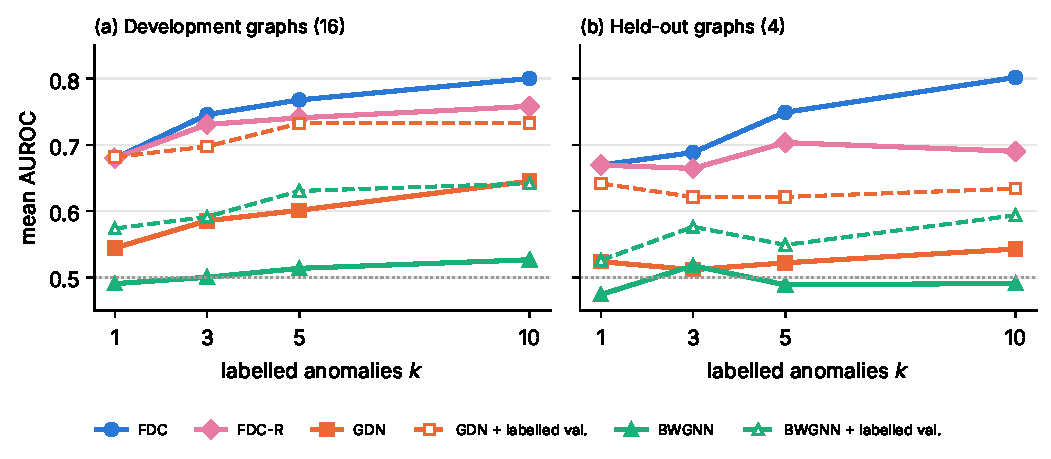
\includegraphics[width=\textwidth]{fig/Fig3_auroc_vs_k.pdf}
\caption{Mean AUROC against the number of labelled anomalies. Dashed lines: baselines with a labelled validation set (20\% of the nodes). Means at each $k$ are over the graphs with enough anomalies (Disney is excluded for $k\ge5$, Enron for $k\ge3$). The dotted line marks random ranking.}
\label{fig:k}
\end{figure}

Table~\ref{tab:pergraph} reports per-graph results at $k=10$. FDC is strongest on the injected-anomaly graphs (0.70--0.97) and on Amazon, Amazon-all and Weibo (0.90--0.95), where the attribute statistics add most to FDC-R (for example 0.682 to 0.899 on Amazon). It loses to the official baselines on three graphs: Facebook, where GDN is almost perfect (0.992 against 0.972); Questions (0.579 against 0.612); and Tolokers (0.645 against 0.661). Questions, Tolokers, Reddit and YelpChi-all remain hard for every method. BWGNN's last-epoch scores are often below 0.5. With few positives and every other node treated as negative, it fits the labelled anomalies' neighbourhoods rather than the anomaly pattern; its validation-selected variant partly repairs this.

\begin{table}[!ht]
\caption{AUROC on the development graphs at $k=10$ (mean, with standard deviation over five seeds for the three main methods). $^{\ast}$Disney has six anomalies and is shown at $k=3$. Bold: best of FDC, GDN and BWGNN.}
\label{tab:pergraph}
\scriptsize
\setlength{\tabcolsep}{2.4pt}
\begin{tabular*}{\textwidth}{@{\extracolsep{\fill}}llcccccccc@{}}
\toprule
Graph & Type & Fixed & FDC-R & FDC & GDN & BWGNN & GDN$^{\dagger}$ & BWGNN$^{\dagger}$ \\
\midrule
Cora & inj. & 0.782 & 0.922 & \textbf{0.919}\,{\tiny$\pm$0.018} & 0.731\,{\tiny$\pm$0.032} & 0.387\,{\tiny$\pm$0.093} & 0.769 & 0.554 \\
CiteSeer & inj. & 0.850 & 0.936 & \textbf{0.931}\,{\tiny$\pm$0.018} & 0.674\,{\tiny$\pm$0.057} & 0.416\,{\tiny$\pm$0.095} & 0.772 & 0.575 \\
PubMed & inj. & 0.847 & 0.930 & \textbf{0.938}\,{\tiny$\pm$0.015} & 0.628\,{\tiny$\pm$0.049} & 0.409\,{\tiny$\pm$0.105} & 0.680 & 0.527 \\
ACM & inj. & 0.759 & 0.916 & \textbf{0.909}\,{\tiny$\pm$0.038} & 0.570\,{\tiny$\pm$0.053} & 0.437\,{\tiny$\pm$0.077} & 0.706 & 0.460 \\
BlogCatalog & inj. & 0.640 & 0.727 & \textbf{0.711}\,{\tiny$\pm$0.048} & 0.581\,{\tiny$\pm$0.050} & 0.359\,{\tiny$\pm$0.070} & 0.611 & 0.494 \\
Flickr & inj. & 0.702 & 0.751 & \textbf{0.703}\,{\tiny$\pm$0.066} & 0.530\,{\tiny$\pm$0.038} & 0.273\,{\tiny$\pm$0.037} & 0.647 & 0.490 \\
Facebook & inj. & 0.876 & 0.933 & 0.972\,{\tiny$\pm$0.013} & \textbf{0.992}\,{\tiny$\pm$0.002} & 0.930\,{\tiny$\pm$0.018} & 0.991 & 0.739 \\
Reddit & org. & 0.573 & 0.520 & \textbf{0.575}\,{\tiny$\pm$0.026} & 0.536\,{\tiny$\pm$0.046} & 0.544\,{\tiny$\pm$0.034} & 0.596 & 0.560 \\
Amazon & org. & 0.720 & 0.682 & \textbf{0.899}\,{\tiny$\pm$0.035} & 0.648\,{\tiny$\pm$0.068} & 0.762\,{\tiny$\pm$0.069} & 0.816 & 0.875 \\
Disney$^{\ast}$ & org. & 0.573 & 0.505 & 0.481\,{\tiny$\pm$0.172} & 0.412\,{\tiny$\pm$0.064} & \textbf{0.553}\,{\tiny$\pm$0.172} & 0.499 & 0.547 \\
Weibo & org. & 0.432 & 0.906 & \textbf{0.948}\,{\tiny$\pm$0.012} & 0.884\,{\tiny$\pm$0.062} & 0.330\,{\tiny$\pm$0.078} & 0.976 & 0.921 \\
Tolokers & org. & 0.386 & 0.604 & 0.645\,{\tiny$\pm$0.046} & 0.653\,{\tiny$\pm$0.074} & \textbf{0.661}\,{\tiny$\pm$0.032} & 0.709 & 0.682 \\
Amazon-all & org. & 0.760 & 0.784 & \textbf{0.905}\,{\tiny$\pm$0.018} & 0.439\,{\tiny$\pm$0.189} & 0.763\,{\tiny$\pm$0.098} & 0.801 & 0.888 \\
YelpChi & org. & 0.440 & 0.719 & \textbf{0.765}\,{\tiny$\pm$0.026} & 0.702\,{\tiny$\pm$0.054} & 0.632\,{\tiny$\pm$0.036} & 0.718 & 0.624 \\
YelpChi-all & org. & 0.500 & 0.511 & \textbf{0.603}\,{\tiny$\pm$0.049} & 0.497\,{\tiny$\pm$0.011} & 0.551\,{\tiny$\pm$0.017} & 0.520 & 0.642 \\
Questions & org. & 0.553 & 0.530 & 0.579\,{\tiny$\pm$0.055} & \textbf{0.612}\,{\tiny$\pm$0.042} & 0.444\,{\tiny$\pm$0.027} & 0.679 & 0.596 \\
\botrule
\end{tabular*}
\end{table}

\subsection{Confirmatory test on held-out graphs}\label{sec:heldout}

Table~\ref{tab:heldout} reports the held-out test, run once with the frozen method. All three confirmatory claims hold. FDC's mean AUROC is 0.723, against 0.546 for the better baseline per combination (C1); it beats both baselines in all 13 combinations (C2); and it exceeds FDC-R (0.681; C3). It also beats the baselines with a labelled validation set in 9 of 13 combinations. Two results qualify this. First, FDC's mean AP on the held-out graphs (0.225) is below FDC-R's (0.252), although its AUROC is higher; AP was not among the confirmatory claims. Second, on Coauthor-CS the attribute statistics slightly lower AUROC at $k\ge3$ (for example 0.939 against 0.963 at $k=3$). With a single labelled anomaly, Books is close to random for every method and Amazon-Photo stays below 0.61, which is what Theorem~\ref{thm:anomaly} predicts when the margins of the statistics are small relative to one shot.

\begin{table}[!ht]
\caption{Confirmatory test on the held-out graphs (AUROC unless stated). The method was frozen before any label of these graphs was read. Bold: best of the four methods without extra labels.}
\label{tab:heldout}
\footnotesize
\begin{tabular*}{\textwidth}{@{\extracolsep{\fill}}lccccccc@{}}
\toprule
Graph & $k$ & FDC & FDC-R & GDN & BWGNN & GDN$^{\dagger}$ & BWGNN$^{\dagger}$ \\
\midrule
Coauthor-CS & 1 & \textbf{0.939} & \textbf{0.939} & 0.522 & 0.422 & 0.741 & 0.564 \\
Coauthor-CS & 3 & 0.939 & \textbf{0.963} & 0.548 & 0.455 & 0.746 & 0.599 \\
Coauthor-CS & 5 & 0.960 & \textbf{0.973} & 0.542 & 0.434 & 0.707 & 0.521 \\
Coauthor-CS & 10 & 0.969 & \textbf{0.972} & 0.596 & 0.341 & 0.756 & 0.583 \\
Amazon-Photo & 1 & \textbf{0.580} & \textbf{0.580} & 0.505 & 0.477 & 0.609 & 0.473 \\
Amazon-Photo & 3 & \textbf{0.582} & 0.534 & 0.540 & 0.560 & 0.610 & 0.582 \\
Amazon-Photo & 5 & \textbf{0.642} & 0.639 & 0.558 & 0.515 & 0.602 & 0.574 \\
Amazon-Photo & 10 & \textbf{0.712} & 0.634 & 0.596 & 0.633 & 0.611 & 0.681 \\
Books & 1 & \textbf{0.505} & \textbf{0.505} & 0.485 & 0.502 & 0.576 & 0.503 \\
Books & 3 & \textbf{0.544} & 0.496 & 0.447 & 0.538 & 0.508 & 0.549 \\
Books & 5 & \textbf{0.645} & 0.498 & 0.466 & 0.518 & 0.554 & 0.552 \\
Books & 10 & \textbf{0.724} & 0.464 & 0.437 & 0.499 & 0.535 & 0.517 \\
Enron & 1 & \textbf{0.653} & \textbf{0.653} & 0.582 & 0.495 & 0.640 & 0.564 \\
\midrule
Mean AUROC & & 0.723 & 0.681 & 0.525 & 0.491 & 0.630 & 0.558 \\
Mean AP & & 0.225 & 0.252 & 0.044 & 0.069 & 0.048 & 0.136 \\
\botrule
\end{tabular*}
\end{table}

\subsection{Statistical significance}\label{sec:signif}

Table~\ref{tab:wilcoxon} tests whether FDC beats each comparison method across graph and shot-size combinations, with the one-sided Wilcoxon signed-rank test on the per-combination mean AUROC \citep{wilcoxon1945individual,demsar2006statistical}. On the held-out graphs FDC is significantly better than both official baselines ($p=0.0001$), and also than both baselines with labelled validation ($p\le0.007$). Pooled over all 75 combinations, every difference is significant at $p<0.002$. The comparison with FDC-R has many ties, because the two methods coincide for $k<3$. The development-graph tests are reported for completeness; they are not independent of method development, and the held-out tests carry the evidential weight.

\begin{table}[!ht]
\caption{One-sided Wilcoxon signed-rank tests of FDC against each method over (graph, $k$) combinations: mean AUROC difference, combinations won, and $p$-value.}
\label{tab:wilcoxon}
\footnotesize
\setlength{\tabcolsep}{2.5pt}
\begin{tabular*}{\textwidth}{@{\extracolsep{\fill}}lccccccccc@{}}
\toprule
 & \multicolumn{3}{c}{Held-out (13)} & \multicolumn{3}{c}{Development (62)} & \multicolumn{3}{c}{All (75)} \\
\cmidrule(lr){2-4}\cmidrule(lr){5-7}\cmidrule(l){8-10}
vs. & $\Delta$AUROC & Wins & $p$ & $\Delta$AUROC & Wins & $p$ & $\Delta$AUROC & Wins & $p$ \\
\midrule
GDN & +0.198 & 13/13 & 0.0001 & +0.154 & 49/62 & $<10^{-8}$ & +0.162 & 62/75 & $<10^{-11}$ \\
BWGNN & +0.231 & 13/13 & 0.0001 & +0.240 & 56/62 & $<10^{-10}$ & +0.238 & 69/75 & $<10^{-12}$ \\
GDN$^{\dagger}$ & +0.092 & 10/13 & 0.0067 & +0.037 & 38/62 & 0.0037 & +0.046 & 48/75 & 0.0003 \\
BWGNN$^{\dagger}$ & +0.164 & 12/13 & 0.0006 & +0.139 & 47/62 & $<10^{-6}$ & +0.143 & 59/75 & $<10^{-8}$ \\
FDC-R & +0.042 & 6/13 & 0.0488 & +0.021 & 26/62 & 0.0082 & +0.024 & 32/75 & 0.0018 \\
\botrule
\end{tabular*}
\end{table}

\subsection{Ablation and development history}\label{sec:ablation}

Table~\ref{tab:ablation} lists every variant evaluated during development, in the order in which the rounds were run. Calibrating directions from the shots is the largest single gain (0.651 to 0.717 mean AUROC), and weighting by the estimated separation adds a further 0.010. Pooling attribute statistics helps organic graphs substantially (0.630 to 0.684) but hurts injected graphs and $k=1$; the null-shrinkage threshold recovers part of the injected loss, and sparse top-8 selection does not help. Gating the attribute statistics by $k$ keeps the organic gain and the $k=1$ performance of FDC-R. Because these variants were chosen on the development graphs, their differences should be read as development evidence; the held-out test of Section~\ref{sec:heldout} is the unbiased estimate of the final method.

\begin{table}[!ht]
\caption{All variants evaluated during development (mean AUROC over the development graphs). R1--R3: development round. Inj./Org.: injected and organic graphs.}
\label{tab:ablation}
\scriptsize
\setlength{\tabcolsep}{2.2pt}
\begin{tabular*}{\textwidth}{@{\extracolsep{\fill}}p{4.6cm}cccccccc@{}}
\toprule
Variant & Round & All & Inj. & Org. & $k{=}1$ & $k{=}3$ & $k{=}5$ & $k{=}10$ \\
\midrule
Fixed directions (no shots) & -- & 0.651 & 0.779 & 0.546 & 0.648 & 0.649 & 0.655 & 0.655 \\
Shot-calibrated directions, relational only & R1 & 0.717 & 0.830 & 0.623 & 0.669 & 0.722 & 0.729 & 0.748 \\
+ separation weights (FDC-R) & R1 & 0.727 & 0.843 & 0.630 & 0.680 & 0.731 & 0.741 & 0.758 \\
+ attribute statistics, pooled & R2 & 0.738 & 0.804 & 0.684 & 0.655 & 0.742 & 0.766 & 0.796 \\
+ null-shrinkage $\tau_k$ & R2 & 0.740 & 0.819 & 0.675 & 0.654 & 0.746 & 0.768 & 0.800 \\
+ top-8 selection & R2 & 0.730 & 0.813 & 0.662 & 0.638 & 0.735 & 0.759 & 0.794 \\
Max of FDC-R and attribute score & R3 & 0.733 & 0.832 & 0.651 & 0.681 & 0.735 & 0.749 & 0.770 \\
$k$-gated: FDC-R if $k<3$, else pooled+shrinkage (FDC) & R3 & 0.747 & 0.830 & 0.679 & 0.680 & 0.746 & 0.768 & 0.800 \\
\botrule
\end{tabular*}
\end{table}

\subsection{Runtime}\label{sec:runtime}

Table~\ref{tab:runtime} reports wall-clock times on the same two-core machine for one run at the largest valid $k$. FDC's time is dominated by computing the statistics, from 0.05\,s on Disney to 111\,s on Amazon-all ($4.4\times10^6$ edges); calibration with the labelled anomalies takes at most 0.24\,s on any graph. The official GDN, whose model is a two-layer linear network on precomputed propagated features, is faster on most graphs. The practical advantage of FDC is therefore not speed of a single run: it needs no training, and once the statistics are computed, adding or correcting labelled anomalies costs a fraction of a second.

\begin{table}[!ht]
\caption{Wall-clock time in seconds for one run (seed 11, largest valid $k$) on a two-core machine. FDC statistics: relational and attribute statistics (computed once per graph); FDC calibration: orientation, weighting and scoring with the labelled anomalies.}
\label{tab:runtime}
\footnotesize
\begin{tabular*}{\textwidth}{@{\extracolsep{\fill}}lrrrrr@{}}
\toprule
Graph & Nodes & Edges & FDC statistics & FDC calibration & GDN (official) \\
\midrule
Disney & 124 & 335 & 0.05 & 0.004 & 0.11 \\
Books & 1,418 & 3,695 & 0.49 & 0.012 & 0.25 \\
CiteSeer & 3,327 & 5,077 & 2.19 & 0.015 & 1.87 \\
Cora & 2,708 & 5,802 & 1.65 & 0.014 & 10.77 \\
Facebook & 1,081 & 27,552 & 0.67 & 0.007 & 0.32 \\
PubMed & 19,717 & 46,423 & 7.03 & 0.080 & 1.44 \\
YelpChi & 23,831 & 49,315 & 6.91 & 0.088 & 0.89 \\
ACM & 16,484 & 74,073 & 34.16 & 0.071 & 14.58 \\
Reddit & 10,984 & 78,516 & 5.13 & 0.039 & 0.55 \\
Coauthor-CS & 18,333 & 83,993 & 32.56 & 0.088 & 12.53 \\
Amazon-Photo & 7,650 & 120,653 & 5.79 & 0.041 & 0.99 \\
Questions & 48,921 & 153,540 & 18.13 & 0.210 & 2.70 \\
BlogCatalog & 5,196 & 172,779 & 32.84 & 0.031 & 17.17 \\
Amazon & 10,224 & 175,608 & 4.13 & 0.046 & 0.54 \\
Enron & 13,533 & 176,987 & 7.03 & 0.058 & 0.67 \\
Flickr & 7,575 & 241,301 & 64.70 & 0.038 & 35.23 \\
Weibo & 8,405 & 377,271 & 9.98 & 0.038 & 1.14 \\
Tolokers & 11,758 & 519,000 & 10.77 & 0.051 & 0.87 \\
YelpChi-all & 45,954 & 3,846,979 & 36.45 & 0.240 & 4.22 \\
Amazon-all & 11,944 & 4,398,392 & 110.93 & 0.054 & 3.03 \\
\botrule
\end{tabular*}
\end{table}

\section{Discussion}\label{sec:discussion}

\paragraph{What the theory explains.} The results follow the asymmetry of Section~\ref{sec:theory}. Unlabelled data cannot orient a statistic (Theorem~\ref{thm:nonid}), which is why no label-free rule transferred. Labelled normal nodes look like the graph as a whole when anomalies are rare (Theorem~\ref{thm:normal}), which is why normal-shot rules stayed near chance. Labelled anomalies identify the direction at an exponential rate in $k$ (Theorem~\ref{thm:anomaly}), which is why FDC improves steadily with $k$ while its error on statistics with large margins vanishes. The observed direction errors stay within the bounds in every case (Table~\ref{tab:bound}).

\paragraph{Why the baselines struggle.} GDN and BWGNN learn a scoring function from the labelled anomalies, with all other nodes treated as normal. With one to ten positives, that function is easily fitted to features of the particular shots; BWGNN's last-epoch AUROC is below 0.5 on most graphs. FDC learns far less: one direction and one weight per statistic, each estimated by an average of $k$ bounded numbers. This low-variance estimate is what makes few shots sufficient, and it is also what limits FDC when no statistic carries the anomaly signal, as on Questions and Tolokers.

\paragraph{Implications for few-shot evaluation.} Generalist detectors are usually evaluated with a few labelled normal nodes. Our results suggest that, for detectors built on statistics, a few labelled anomalies are far more informative, and that few-shot protocols should include them. They also suggest that the orientation of each statistic should be reported as an explicit assumption of any training-free detector.

\paragraph{Limitations.} FDC is built on one family of statistics; it inherits their blind spots, and on graphs without informative statistics (Reddit, Questions) every method stays close to random. The held-out test contains four graphs and 13 combinations; it is a clean test, but a small one. The held-out graphs had been evaluated once before, in the label-free rule study, although not during FDC's development. Meta-GDN, which needs labelled auxiliary graphs in the same feature space, was not compared, and recent semi-supervised detectors beyond GDN and BWGNN were not run. The baselines were run with their official settings, without tuning; with a labelled validation set they improve, and we report that variant throughout. Finally, FDC's held-out AP is slightly lower than that of its relational-only variant, and it is not faster than GDN for a single run.

\section{Conclusion}\label{sec:conclusion}

Training-free graph anomaly detectors depend on a choice that unlabelled data cannot make: which tail of each statistic is anomalous. We proved that labelled normal nodes barely help with this choice when anomalies are rare, and that a few labelled anomalies settle it at an exponential rate. Few-shot direction calibration turns this into a method with no trainable parameters. Evaluated against the official GDN and BWGNN under identical supervision, with protocols fixed in advance and a held-out confirmatory test, it was better on most development graphs and on every held-out combination. The results argue for treating orientation as an explicit, testable part of statistic-based detectors and for including labelled anomalies in few-shot evaluation.

\backmatter

\bmhead{Acknowledgements}
Not applicable.

\section*{Declarations}

\begin{itemize}
\item \textbf{Funding:} This research did not receive external funding.
\item \textbf{Competing interests:} The authors declare no competing interests.
\item \textbf{Ethics approval and consent to participate:} Not applicable.
\item \textbf{Data availability:} All datasets are public. Benchmark files were obtained from the repositories of ARC (\url{https://github.com/yixinliu233/ARC}), UNPrompt (\url{https://github.com/mala-lab/UNPrompt}), TAM (\url{https://github.com/mala-lab/TAM-master}), CARE-GNN (\url{https://github.com/YingtongDou/CARE-GNN}), PyGOD (\url{https://github.com/pygod-team/data}) and the Planetoid repository.
\item \textbf{Code availability:} Code, protocols with their hashes, the freeze record, per-run results and the scripts that generate every table and figure are available at \url{https://github.com/khanwasim051/direction-identifiability-gad}.
\item \textbf{Use of large language models:} An AI assistant (Claude, Anthropic) was used to help implement the statistics, the method and the experiment scripts, run experiments, derive and check proofs, and draft and edit the manuscript. The authors designed the study, approved every protocol before it was run, checked the results against the result files, and take responsibility for the content.
\item \textbf{Author contributions:} Wasim Khan conceived the study, implemented the methods, carried out the experiments and analysis, and wrote the main manuscript text. Shaikh Abdul Waheed contributed to the conceptualization and supervised the work. Sujit R. Wakchaure contributed to the methodology and analysed the results. Anjali Devi Patil analysed the results and edited the manuscript. Deepti Varshney carried out the literature review and prepared the figures. Vajid Khan organized the datasets and contributed to the visualization. All authors reviewed and approved the final manuscript.
\end{itemize}

\begin{appendices}

% ---------------------------------------------------------------------------
% Appendix: proofs for Section \ref{sec:theory}
% ---------------------------------------------------------------------------
\section{Proofs}\label{app:proofs}

Throughout, $c(i,l) = \mathbb{1}[t_l < t_i] + \tfrac12\mathbb{1}[t_l = t_i]$, so that $c(i,l) + c(l,i) = 1$ and $c(i,i) = \tfrac12$.

\begin{proof}[Proof of Lemma~\ref{lem:sign}]
By \eqref{eq:rankpos}, $U_i = \frac1n\sum_{l\in V} c(i,l)$. Splitting the inner sum into anomalies and normal nodes,
\[
m\,\mu = \sum_{i\in\mathcal{A}} U_i
= \frac1n\Big(\sum_{i\in\mathcal{A}}\sum_{l\in\mathcal{A}} c(i,l) + \sum_{i\in\mathcal{A}}\sum_{l\in\mathcal{N}} c(i,l)\Big)
= \frac1n\Big(\frac{m^2}{2} + m(n-m)\,\mathrm{AUC}\Big),
\]
because the $m^2$ ordered pairs within $\mathcal{A}$ split into pairs $(i,l),(l,i)$ contributing $1$ each and diagonal terms contributing $\tfrac12$ each, for a total of $m^2/2$. Dividing by $m$ gives $\mu = \pi/2 + (1-\pi)\,\mathrm{AUC}$, that is, $\mu - \tfrac12 = (1-\pi)(\mathrm{AUC} - \tfrac12)$. Since $1 - \pi > 0$, $\mu - \tfrac12$ and $\mathrm{AUC} - \tfrac12$ have the same sign.
\end{proof}

\begin{proof}[Proof of Theorem~\ref{thm:nonid}]
With distinct values, every node in $\mathcal{A}_\uparrow$ has a larger value than every node outside it, so labelling $\mathcal{A}_\uparrow$ as anomalous gives $\mathrm{AUC} = 1$; symmetrically, labelling $\mathcal{A}_\downarrow$ gives $\mathrm{AUC} = 0$. Both labellings have $m$ anomalies. A label-free rule $\phi$ sees the same input under both, so $p = \Pr[\phi = \text{upper}]$ is the same. Its error is $1 - p$ under the first labelling and $p$ under the second, and $\max(1-p,\,p) \ge \tfrac12$.
\end{proof}

\begin{proof}[Proof of Theorem~\ref{thm:normal}]
Let $M = V \setminus (\mathcal{A}_\uparrow \cup \mathcal{A}_\downarrow)$, $|M| = n - 2m \ge m'$. Under the first labelling the normal nodes are $M \cup \mathcal{A}_\downarrow$; under the second they are $M \cup \mathcal{A}_\uparrow$. Both sets have $n - m$ elements. Let $S$ be the set of $m'$ revealed normal nodes and $E$ the event $S \subseteq M$. Under either labelling,
\[
\Pr[E] = \binom{n-2m}{m'}\Big/\binom{n-m}{m'} = \prod_{i=0}^{m'-1}\frac{n-2m-i}{n-m-i} = q,
\]
and conditionally on $E$, $S$ is a uniform $m'$-subset of $M$ under both labellings. Hence, on $E$, the observed data $(G, S)$ have the same distribution under both labellings, and so does the output of any rule $\phi$. Write $p_E = \Pr[\phi = \text{upper} \mid E]$. Then
\[
\Pr_{\uparrow}[\text{error}] + \Pr_{\downarrow}[\text{error}]
\;\ge\; q\,(1 - p_E) + q\,p_E \;=\; q,
\]
so the larger of the two errors is at least $q/2$. Each factor of the product is at least its last factor, which gives $q \ge \big((n-2m-m'+1)/(n-m-m'+1)\big)^{m'} = \big(1 - m/(n-m-m'+1)\big)^{m'}$. For $m' \ll n$ this is approximately $\big(1-\pi/(1-\pi)\big)^{m'} \approx \exp(-m'\pi/(1-\pi))$.
\end{proof}

\begin{proof}[Proof of Theorem~\ref{thm:anomaly}]
Assume the upper tail is anomalous, so $\mu = \tfrac12 + \Delta$; the other case is symmetric. The rule errs only if $\hat\mu \le \tfrac12$, that is, if $\hat\mu - \mu \le -\Delta$. The shots are drawn without replacement from the finite population $\{U_i : i \in \mathcal{A}\}$, whose values lie in $(0,1)$ and have mean $\mu$ and variance $\sigma^2$. \citet{hoeffding1963probability}, Theorem~4, shows that for every continuous convex function $f$, $\mathbb{E} f(\sum_s U_{a_s})$ under sampling without replacement is at most its value under sampling with replacement. Every exponential-moment (Chernoff) bound for independent draws therefore also holds here. Hoeffding's inequality for independent variables with range $1$ gives $\Pr[\hat\mu - \mu \le -\Delta] \le \exp(-2k\Delta^2)$. Bernstein's inequality, with variance $\sigma^2$ and $|U_{a_s} - \mu| \le 1$, gives $\Pr[\hat\mu - \mu \le -\Delta] \le \exp\!\big(-k\Delta^2 / (2\sigma^2 + 2\Delta/3)\big)$. Both are derived from exponential moments, so both apply.
\end{proof}

\begin{proof}[Proof of Corollary~\ref{cor:k}]
By Theorem~\ref{thm:anomaly} and a union bound over the $J$ statistics, the probability that at least one direction is wrong is at most $J\exp(-2k\Delta_{\min}^2)$. This is at most $\varepsilon$ when $k \ge \ln(J/\varepsilon)/(2\Delta_{\min}^2)$.
\end{proof}

\begin{proof}[Proof of Proposition~\ref{prop:tau}]
With distinct values, the rank positions are $\{(i-\tfrac12)/n : i = 1,\dots,n\}$, with mean exactly $\tfrac12$ and variance $(n^2-1)/(12n^2) < 1/12$. The upper evidence is $U$ and the lower evidence $1-U$, so both have this mean and variance. The two-sided evidence is $|r| = |2U - 1|$. It has mean $\tfrac12$ for even $n$ (and $\tfrac12 - 1/(2n^2)$ for odd $n$), and its second moment equals that of $r$, namely $(n^2-1)/(3n^2)$, so its variance is at most $1/12$. Ties only reduce these variances. If the $k$ shots are a uniform random sample of nodes, the shot mean of each evidence therefore has expectation $\tfrac12 + O(1/n)$ and variance at most $1/(12k)$. This holds with replacement; sampling without replacement multiplies the variance by the finite-population factor $(n-k)/(n-1) \le 1$. Hence its standard deviation is at most $\tau_k = 1/\sqrt{12k}$.

For the second claim, let statistic $j$ have margin $\Delta_j > \tau_k$, and say its upper tail is anomalous. The estimated separation of the chosen tail is at least that of the upper tail, $\hat s_j \ge \hat\mu - \tfrac12$. The weight is zero only if $\hat s_j \le \tau_k$, which implies $\hat\mu - \mu \le -(\Delta_j - \tau_k)$. By the Hoeffding step in the proof of Theorem~\ref{thm:anomaly}, this has probability at most $\exp(-2k(\Delta_j - \tau_k)^2)$.
\end{proof}

\section{Protocols and freeze record}\label{app:prereg}

Table~\ref{tab:hashes} lists the protocol files of this study, each written before the results it governs were computed, with their SHA-256 hashes. The freeze record stores the hashes of the method code (\texttt{fsdc.py}, \texttt{step2.py}, \texttt{step3.py}), of the base detector's implementation and of all protocols. The confirmatory script refuses to run if any of these files has changed. The held-out labels are stored separately from the development labels.

\begin{table}[h]
\caption{Protocol files and their SHA-256 hashes (first 16 hexadecimal digits).}
\label{tab:hashes}
\footnotesize
\begin{tabular}{@{}lll@{}}
\toprule
Stage & File & SHA-256 \\
\midrule
Round 1: feasibility, go/no-go & \texttt{FEASIBILITY\_PROTOCOL.md} & \texttt{5b71e1d64bd59095} \\
Official baselines & \texttt{BASELINES2\_PROTOCOL.md} & \texttt{d548b49fbc668f70} \\
Round 2: attribute statistics & \texttt{STEP2\_PROTOCOL.md} & \texttt{59bad00040df7c47} \\
Round 3: final variants & \texttt{STEP3\_PROTOCOL.md} & \texttt{6a8f5c5455e2fd32} \\
Confirmatory test & \texttt{CONFIRMATORY\_PROTOCOL.md} & \texttt{f75b980c629185f2} \\
\botrule
\end{tabular}
\end{table}

\end{appendices}

\bibliography{refs}

\end{document}
